\section{Electronic Mail}
Electronic Mail \citep[Chapter 11]{redhatemail} is a communication service which has been used since 1971 \citep{wikiemail} when the first network email with the text ``QWERTYUIOP'' was sent through ARPAnet (Advanced Research Projects Agency Network, the first network which implements the TCP/IP protocol) with the experimental protocol CYPNET. Nowadays, the messages are delivered by using a client/server architecture. In this way, an email is created by using a client-side mail program. Then, this software sends the message to a server, which will redirect to the recipient's mail server. From it, the email is going to be provided to the addressee.

In order to make all this process possible, a wide range of standard network protocols exists for allowing different machines (often they execute distinct operative systems and make use of different mail programs) to share emails. In this section, we are going to study these protocols and the API which is going to be used for reading, sending emails and accessing to the user's email data. First of all, we are going to explain the main email management protocols, both electronic mail transmission protocol (such as Simple Mail Transfer Protocol, which is explained in Section \ref{ssect:smtp}) and message access protocol (such as Internet Message Access Protocol and Post Office Protocol, which are studied in Sections \ref{ssect:imap} and \ref{ssect:pop}, respectively). 

In spite of being a mail server-independent solution, as we will see, we are going to find security issues which are going to hinder our user's email data access. These trials come from the automatic server access. For this reason, Gmail API is going to be introduced (see Section \ref{ssect:gmailapi}) and, finally, the assessment of the advantages and disadvantages of making use of the email protocols or the Gmail API is discussed (see Section \ref{ssect:protvsapi}).

\subsection{Simple Mail Transfer Protocol} \label{ssect:smtp}

Simple Mail Transfer Protocol (also known as SMTP) is a network connection-oriented communication protocol used for the exchange of e-mail messages. It was originally defined in \cite{rfc821} (for the transfer) and in \cite{rfc822} (for the message). It is currently defined in \cite{rfc5321} and \cite{rfc5322}. However, this protocol has some limitations when it comes to receiving messages on the destination server. For this reason, this task is intended for other protocols such as the Internet Message Access Protocol (see Section \ref{ssect:imap}) or the Post Office Protocol (refer to Section \ref{ssect:pop}), and SMTP is used specifically to send messages.

Making use of SMTP, an email is ``pushed'' from one mail server to another (next-hop mail server) until it reaches its destination. The message is not routed according to the message recipients specified during the client's connection to the SMTP server, but from the destination mail server. Thanks to the fact that this protocol has a feature to initiate mail queue processing, an intermittently connected mail server can extract messages from another remote server when necessary.

\subsection{Post Office Protocol} \label{ssect:pop}

Post Office Protocol (also known as POP) is an application protocol (in OSI Model) for obtaining e-mails stored in a remote Internet server called POP server. It was originally defined in \cite{rfc918} (it was POP version 1, also known as POP1). Current POP version (POP3, in general when we talk about POP we refer to this version) is detailed in \cite{rfc1939}.

POP was designed for receiving emails. Using POP, users with intermittent or very slow Internet connections (such as modem connections) can download their email while online and check it later even when offline. The general operation is: a client using POP3 connects, gets all messages, stores them on the user's computer as new messages, deletes them from the server, and finally disconnects. However some mail clients include the option to leave messages on the server. They use the order UIDL (Unique IDentification Listing) which, unlike most POP3 commands, does not identify messages depending on their mail server ordinal number. This results from the fact that the mail server ordinal number creates problems when a client tries to leave messages on the server, since messages with numbers change from one connection to the server to another. Accordingly, server which makes use of UIDL, assigns a unique and permanent character string to each message. Thus, when a POP3-compatible mail client connects to the server, it uses the UIDL command to map the message identifier. This way the client can use that mapping to determine which messages to download and which to save at the time of downloading.

Like other old Internet protocols, POP3 used a signature mechanism without encryption. The transmission of POP3 passwords in plain text still occurs. Nowadays POP3 has various authentication methods that offer a diverse range of levels of protection against illegal access to users' mailboxes.

The advantage over other protocols is that between server-client you do not have to send so many commands for communication between them. The POP protocol also works properly if you do not use a constant connection to the Internet or to the network that contains the mail server.

\subsection{Internet Message Access Protocol} \label{ssect:imap}

Internet Message Access Protocol (also known as IMAP) is an application protocol, designed as an alternative to Post Office Protocol (se Section \ref{ssect:pop}) in 1986, which allows the access to stored messages in an Internet server. As with the Post Office Protocol, with IMAP you can access your e-mail from any computer with an Internet connection. The current version of IMAP (IMAP version 4 review 1 or IMAP4rev1) is defined in \cite{rfc3501}.

In contrast to Post Office Protocol, IMAP allows multiple clients to manage the same mailbox. This fact results from the main differences between these two protocols: IMAP does not remove email from server until the client specifically requests it (as POP removes them by default, it is impossible to accessing them from another device which has not the downloaded messages) and it does not download the messages to the user's computer (clients may optionally store a local copy of them). This last property gives raise to several advantages with regard to Post Office Protocol: the immediate notification of the arrival of a mail (due to it works in permanent connection mode) while POP checks if there are new e-mails every few minutes (which causes an appreciable rise in traffic and in the time the user has to wait to send a request to the server, because it is necessary to complete the download of all new messages first), it is possible to create shared folders with other users (it depends on the mail server), the e-mails do not take up memory in the user's local device while POP downloads them regardless of whether they are going to be read or not (effectively IMAP has to download a message when it is going to be read, but they are temporary files and only the e-mail headers are downloaded to manage the mailbox) and it allows the user to manage folders, templates and drafts in server in addition to be able to search a mail from keywords.

\subsection{Gmail API}\label{ssect:gmailapi}
As we will see in Section \ref{ssect:protvsapi}, due to the automatic server access, directly using the communication protocol for electronic mail transmission (SMTP) and for retrieving email messages from a mail server (POP or IMAP) will cause us security problems in accessing the user's email data. For this reason, we are going to make use of Gmail API. In this section we are going to study it. Thus in Section \ref{sssect:oauth}, we are going to study the necessary protocol for accessing the Gmail API and consequently for being able to get into the user's email data. Further on, we will require a resource (like a programming object) we can work with and how to obtain it is explained in Section \ref{sssect:gmailres}. Once we count on this general resource, we have the necessary tools to be able to understand and handle the internal architecture of the Gmail API and the different means it provides in order to achieve our goal. Therefore, in Sections \ref{sssect:labres}, \ref{sssect:msgres}, \ref{sssect:threads} and \ref{sssect:drafts} we are going to delve into the essential resources for our purpose: labels, messages, threads and drafts, respectively.

Finally, as this API is not the only means of accessing the user's mail data (we have studied other ways in previous sections), we will end with a brief description about the API usage limits (in Section \ref{ssect:apilimits}) to assess its use with respect to other methods of email access.

\subsubsection{OAuth 2.0 Protocol}\label{sssect:oauth}
Open Authorization or OAuth \citep{oauth} is an open standard which allows simple authorization flows for web services or applications. It is a protocol defined in \cite{rfc6749} which allows the site's users to share their information with another site without providing their full identity. This mechanism is used by companies like Google, Facebook, Twitter and Microsoft to allow users to share information about their accounts with third-party applications or websites

Gmail API, as it also happens in the case of other Google APIs, uses OAuth 2.0 protocol \citep{oauthforgoogle} to handle authentication and authorization. It will provide us a secure and trusted login system to access to the user's Gmail data.

The basic working process of OAuth 2.0 protocol can bee seen in Figure \ref{fig:oauth}. As we can observe, at first our application carries out a request in which it sends a token. This token includes, among other things, a credential, which helps Google Servers  to identify the application, and a list of OAuth 2.0 Scopes \citep{oauth-scopes-google}, which are a ``mechanism  in OAuth 2.0 to limit an application's access to a user's account. An application can request one or more scopes. This information is then presented to the user in a consent screen, and the access token issued to the application will be limited to the scopes granted'' \citep{oauth-scopes}. We will use the Gmail API OAuth 2.0 Scope which allows us to read, compose, send, and delete emails.

Once the user has logged in the Gmail account (authentication) and accepted all the necessary permissions that our application needs (authorization), our process receives an authorization code which is going to be exchanged for an access token \citep{oauth-exchange}. Then, we will be in possession of the OAuth 2.0 credentials for the user \citep{oauth2.credentials} which we are going to use for accessing the user's Gmail account.

\begin{figure}[h]
	\centering%
	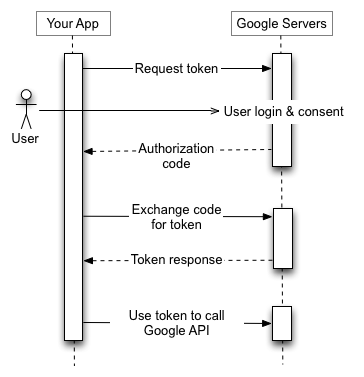
\includegraphics[width = 0.5\textwidth]{Imagenes/Bitmap/webflow.png}%
	\caption{OAuth 2.0 for Web Server Applications and Installed Applications.}%
	Image extracted from \cite{oauthforgoogle}
	\label{fig:oauth}
\end{figure}

\subsection{Advantages and disadvantages of email protocols versus the use of Gmail API} \label{ssect:protvsapi}